\documentclass[11pt]{article}
\usepackage[margin=1in]{geometry}
\usepackage{amsmath,booktabs,graphicx}
\graphicspath{{../figures/}{figures/}}
\title{Comparing Equal-Mass Beam Geometries}
\author{Gabriel Cirker}
\date{}
\begin{document}\maketitle
\begin{abstract}
This study compares the deflection and ideal axial buckling loads of three equal-mass beams. A solid rectangle, a hollow box and a parabolically tapered rectangle are modeled using Euler--Bernoulli beam elements. Under the dimensions chosen here, the hollow section is stiffest, while the tapered beam outperforms the baseline solid beam. These results describe an idealized comparison, not an optimized bridge design.
\end{abstract}
\section{Model and method}
Each steel beam has length $L=1$ m, modulus $E=200$ GPa, density $7850$ kg/m$^3$ and mass 6.28 kg. The solid baseline is 20 mm wide and 40 mm deep. The hollow section has a 40 mm by 60 mm outer envelope and a uniform wall thickness selected to match the baseline area. The tapered section has constant width and depth $h(x)=h_0[1-0.5(2x/L-1)^2]$, with $h_0$ selected to match the mass.

Pinned supports are used at both ends. A transverse load of 1000 N acts at midspan. For variable stiffness the beam equation is $(EI(x)y'')''=q$. Cubic Hermite elements discretize the bending energy, with two-point quadrature. A separate linear elastic eigenvalue analysis estimates the first axial buckling load. Deflection and axial buckling are different load cases.
\section{Results and checks}
\begin{center}\begin{tabular}{lrrr}\toprule
Section & Maximum deflection (mm) & Buckling load (kN) & Load/weight \\\midrule
Solid & 0.9766 & 210.552 & 3418 \\
Hollow & 0.2815 & 730.450 & 11857 \\
Tapered & 0.6880 & 276.663 & 4491 \\\bottomrule\end{tabular}\end{center}
The 80-element solid beam agrees with the closed-form midspan deflection $PL^3/(48EI)$ and Euler load $\pi^2EI/L^2$. For the tapered beam, refining from 40 to 80 elements changes the maximum deflection by less than 0.001\% and the buckling load by less than 0.001\%. These checks support numerical consistency, not experimental validation.
\begin{figure}[ht]\centering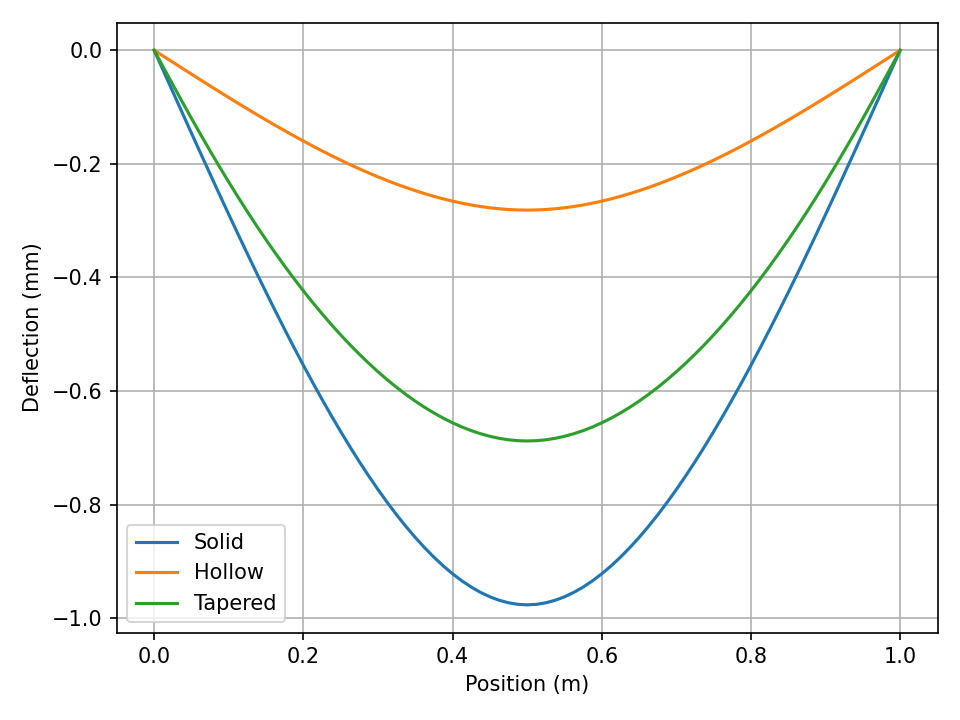
\includegraphics[width=.8\textwidth]{deflection_plot.png}\caption{Deflection under the transverse midpoint load.}\end{figure}
\section{Discussion}
The larger hollow envelope places material farther from the neutral axis and provides the greatest bending stiffness among these particular sections. Its advantage depends on the allowed outer dimensions. The tapered section places more material near midspan, where bending moment is highest. Neither result establishes a global optimum. The load-to-weight ratio uses the ideal axial buckling load and is not a general measure of structural strength. Local wall buckling, yielding, shear deformation, connections, imperfections and fabrication are outside this model. Physical tests and additional design constraints would be needed for a practical bridge comparison.
\end{document}
